%************************************************************************************************************
\section{Computer Simulation and Safety Analysis of Nuclear Power Plant}\label{sec:intro_computer_simulation}
%************************************************************************************************************

%------------------------------------------------------------------------------------------
\subsection{Scientific Computer Simulation}\label{sub:intro_scientific_computer_simulation}
%------------------------------------------------------------------------------------------

% A definition
The ubiquity of computer simulation in science and engineering has resulted in numerous definitions of the term \textit{scientific computer simulation}, \textit{model}, and \textit{simulation}.
\marginpar{scientific computer simulation}
To avoid confusion, this thesis adopts a recent definition proposed by Kaizer et al.\cite{Kaizer2015} quoted below:
\begin{quote}
	Scientific Computer Simulation is the imitation of a behavior of a system, entity, phenomenon, or process in the physical universe 
	using limited mathematical concepts, symbols, and relations through the exercise or use of scientific computer model.
\end{quote}

% The definition, explained
This definition highlights three main points.
\marginpar{model, simulation, scientific simulation, and scientific computer simulation}
First, this definition accentuates the difference between \emph{model} and \emph{simulation}.
A model deals with the notion of representation of a system, while a simulation deals with the notion of imitation of a behavior of that system.
Secondly, a model is said to be scientific when it represents the behavior of a real world system as its subject.
Finally, the modifier \emph{computer} generally implies that the mathematical models cannot be solved analytically and their solutions require a computer.
Though the associated numerical approximations can affect its solution. 
Thus many computational-related aspects often need to be considered.
This thesis only deals with computer simulation.

%The model itself is then referred to as physical model\footnote{Note that this term is referring to the mathematical model of a physical process, and \emph{not} a physical copy of object of interest (vis-à-vis conceptual model). As of October $31$, $2017$ the entry ``physical model'' in Wikipedia, the first hit given by Google, refers to the latter \cite{Wikipedia2017}.} .

% A distinction by Beven
Beven \cite{Beven2009} articulates the definition of a scientific model: a perceptual model (i.e., the theoretical description of the physical phenomena),
a formal model (i.e., its mathematical description),
and a procedural model (i.e., the computer implementation of the formal model).
For many physical models of complex system, only the procedural model is able to make a quantitative prediction of the system behavior.
Thus, these distinctions are useful in acknowledging the level of approximation involved in modeling.

% Code
A computer software that implements scientific models down to the solution algorithms is called a \emph{scientific code} or simply a \emph{code} \cite{Trucano2006}.
\marginpar{Code}
Many modern implementation of scientific codes, apart from possibly being specific to a scientific domain, are comprehensive platforms.
For instance, in the context of \gls[hyper=false]{th} system modeling, such codes allows modeling various attributes of the system ranging from its geometry, initial and boundary conditions, and design variables to the settings for discretization scheme and numerical solver.

% Simulator
A \emph{simulation} or a \emph{calculation} \cite{Trucano2006} using a code can only be made on a particular well-specified system, where all the aforementioned attributes (geometry, initial and boundary conditions, etc.) have been completely fixed or specified.
\marginpar{Simulator}
As a result, the terms \emph{computer simulation model} or \emph{simulator} include not only the code itself, but also the particular system of interest being modeled using the code \cite{OHagan2006}.

%-----------------------------------------------------------------------------------------------------------------------------------
\subsection[Codes and Safety Analysis of Nuclear Power Plant]{Codes and Safety Analysis of Nuclear Power Plant}\label{sub:intro_dsa}
%-----------------------------------------------------------------------------------------------------------------------------------

% Goal of simulation and entry to safety analysis
Scientific codes play a central role in the deterministic safety analysis of an \gls[hyper=false]{npp}.
They provide a \emph{physics-based} evaluation of relevant phenomena taking place in the plant during a broad range of postulated transients to demonstrate that safety requirements of operation are met \cite{IAEA2009}.
The demonstration is carried out with respect to acceptance criteria, a set of limits and conditions ensuring the integrity of the safety barriers.
The criteria are set by regulatory bodies for all operational states of the plant, normal and off-normal.

% Deterministic safety analysis
The physics-based evaluation is achieved by the use of scientific codes to predict the response of the plant to a postulated transient scenario.
In other words, it is achieved through simulation.
\marginpar{Codes in safety analysis of NPP}
As noted in \cite{IAEA2009,DAuria2012}, there are four distinct but related disciplines associated with the different (spatio-temporal) physical processes involved that are important in the analysis of the plant behavior:
the neutronics of the core;
the thermo-mechanics of the fuel and structure;
the radiological analysis of a possible release;
and, the system thermal-hydraulics of the plant, the subject of the present thesis\footnote{Ref.~\cite{DAuria2012} added one additional key discipline, namely: reliability analysis. It is excluded in the above listing as it is not technically a discipline of \emph{physics}.}.
Each of these disciplines (or domains) is, in turn, characterized by a distinct set of governing physical equations of the process involved and thus often analyzed by a distinct code.

% Entry to Conservative vs Best Estimate
The connection between the physics-based evaluation and the de\-monstration of safety is established, among other things, by setting the acceptance criteria in terms of limiting physical quantities relevant for the phenomena involved.
The upper tolerance limit of $1'204\,[^oC]$ for the \glsfirst[hyper=false]{pct} is one such criteria for \glspl[hyper=false]{lwr} \cite{USNRC2017}.
Whether the physical quantities associated with a given plant respect such limits is checked through prediction using simulations. 
Such an analysis based on simulation is conducted using one of two main approaches \cite{IAEA2009} described in the following in the context of system thermal-hydraulics analysis.

% Conservative Analysis
During the early days of reactor safety analysis, prediction using computer model of \gls[hyper=false]{npp} behavior during transient, off-normal or accident conditions, was approached with a high-degree of conservatism.
\marginpar{Conservative analysis}
Conservatism called for the most pessimistic and penalizing modeling assumptions (including the initial and boundary conditions) to ensure conservative results, which is far below their (expected) values in reality.
This approach, though less realistic, was justified by limited modeling capabilities as well as limited knowledge of the physical process involved during those transients.
However, it was later found that there are conditions where conservative assumptions do not necessarily lead to conservative (or even physical) predictions.

% An Illustration
As an example of this contradiction, consider the following situation in the analysis of a \gls[hyper=false]{loca} of an \gls[hyper=false]{lwr} as described in \cite{IAEA2009}.
\marginpar{An illustration}
Assuming less interfacial shear between liquid and gas phases of the coolant (water) reduces mist flow during \gls[hyper=false]{loca} and is conservative in the sense that less heat will be transferred to the coolant flow in the upper region of the core.
This, in turn, penalizes the fuel temperature prediction.
But this assumption also implies that the time to refill the core is shorter as there will be more liquid retained in the reactor cooling system.
Furthermore, with less shear, there is less resistance in injecting emergency coolant into the core (condition known as the counter-current flow limitation).
Both of these are clearly non-conservative and contradicting the initial conservative assumption.

% Best-estimate Analysis
Because of this example and many others \cite{IAEA2009}, a more accurate prediction of two-phase flow transient behavior was deemed necessary for the safety analysis of \gls[hyper=false]{npp}, in particular \gls[hyper=false]{lwr}, under accident conditions.
\marginpar{Best-estimate analysis}
As opposed to the conservative analysis, the term for this approach was coined \emph{best-estimate} analysis.
Such an analysis calls for more physically sound thermal-hydraulics models with more realistic modeling assumptions, which at the same time are also backed by experimental data obtained from numerous experimental programs conducted in Separate and Integral Effect Test Facilities.
With the idea of having more realistic prediction in mind, best-estimate \gls[hyper=false]{th} system codes were developed.
The codes were designed to be comprehensive tools capable of simulating realistically a wide range of transients foreseen in \gls[hyper=false]{lwr} operation,
and were developed using the current best understanding of flow processes expected to happen during the transients.

%--------------------------------------------------------------------------------
\subsection{Thermal-Hydraulics (TH) System Codes}\label{sub:intro_th_system_code}
%--------------------------------------------------------------------------------

% Thermal-Hydraulics System Code, what and why
A \gls[hyper=false]{th} system code is a tool to simulate the flow behavior of the reactor coolant in the entire \gls[hyper=false]{lwr} during wide range of transients foreseen in its operation.
\marginpar{TH system code}
This implies solving time-dependent conservation equations describing the two-phase fluid flow inside the coolant circuit coupled with a heat conduction equation in solid, describing the heat transfer between fluid and heated elements (e.g., fuel rods).
The simulation of the plant behavior also requires an explicit modeling of the geometry, components, equipments, and systems that are specific to \glspl[hyper=false]{lwr} \cite{DAuria2012}.  

% Nodalization
The coolant circuit of a \gls[hyper=false]{npp} is a complex system.
The system includes the reactor pressure vessel and all its intricate contents; kilometers of interconnecting pipes; scores of valves, pumps, and tanks; as well as numerous special components from steam generator to condenser.
\marginpar{Nodalization}
The first major simplification taken for describing the fluid flow in the coolant circuit is by \emph{flow area averaging} (will be detailed further in Chapter~\ref{ch:trace_reflood}). 
This results in $1$-dimensional \emph{nodalization} of the circuit.
Through nodalization, a \gls[hyper=false]{npp} is decomposed into a set of interconnected \emph{nodes} which holds discretized information of fluid flow (see Fig.~\ref{fig:ch1_nodalization}).
Due to the $1$-dimensional simplification of the flow\footnote{Some system codes allow a $3$-dimensional modeling for selected components, mainly the reactor pressure vessel where $3$-dimensional effects might be of relevance to safety analysis. However, as of today, no system code supports full $3$-dimensional modeling of all the components in the coolant circuit.}, a node is only characterized by its \emph{fluid cell} (with attributes of length and free volume) and its \emph{faces} (with attributes of flow area, hydraulic diameter, and orientation). 
\begin{figure}[bth]	
	\centering
	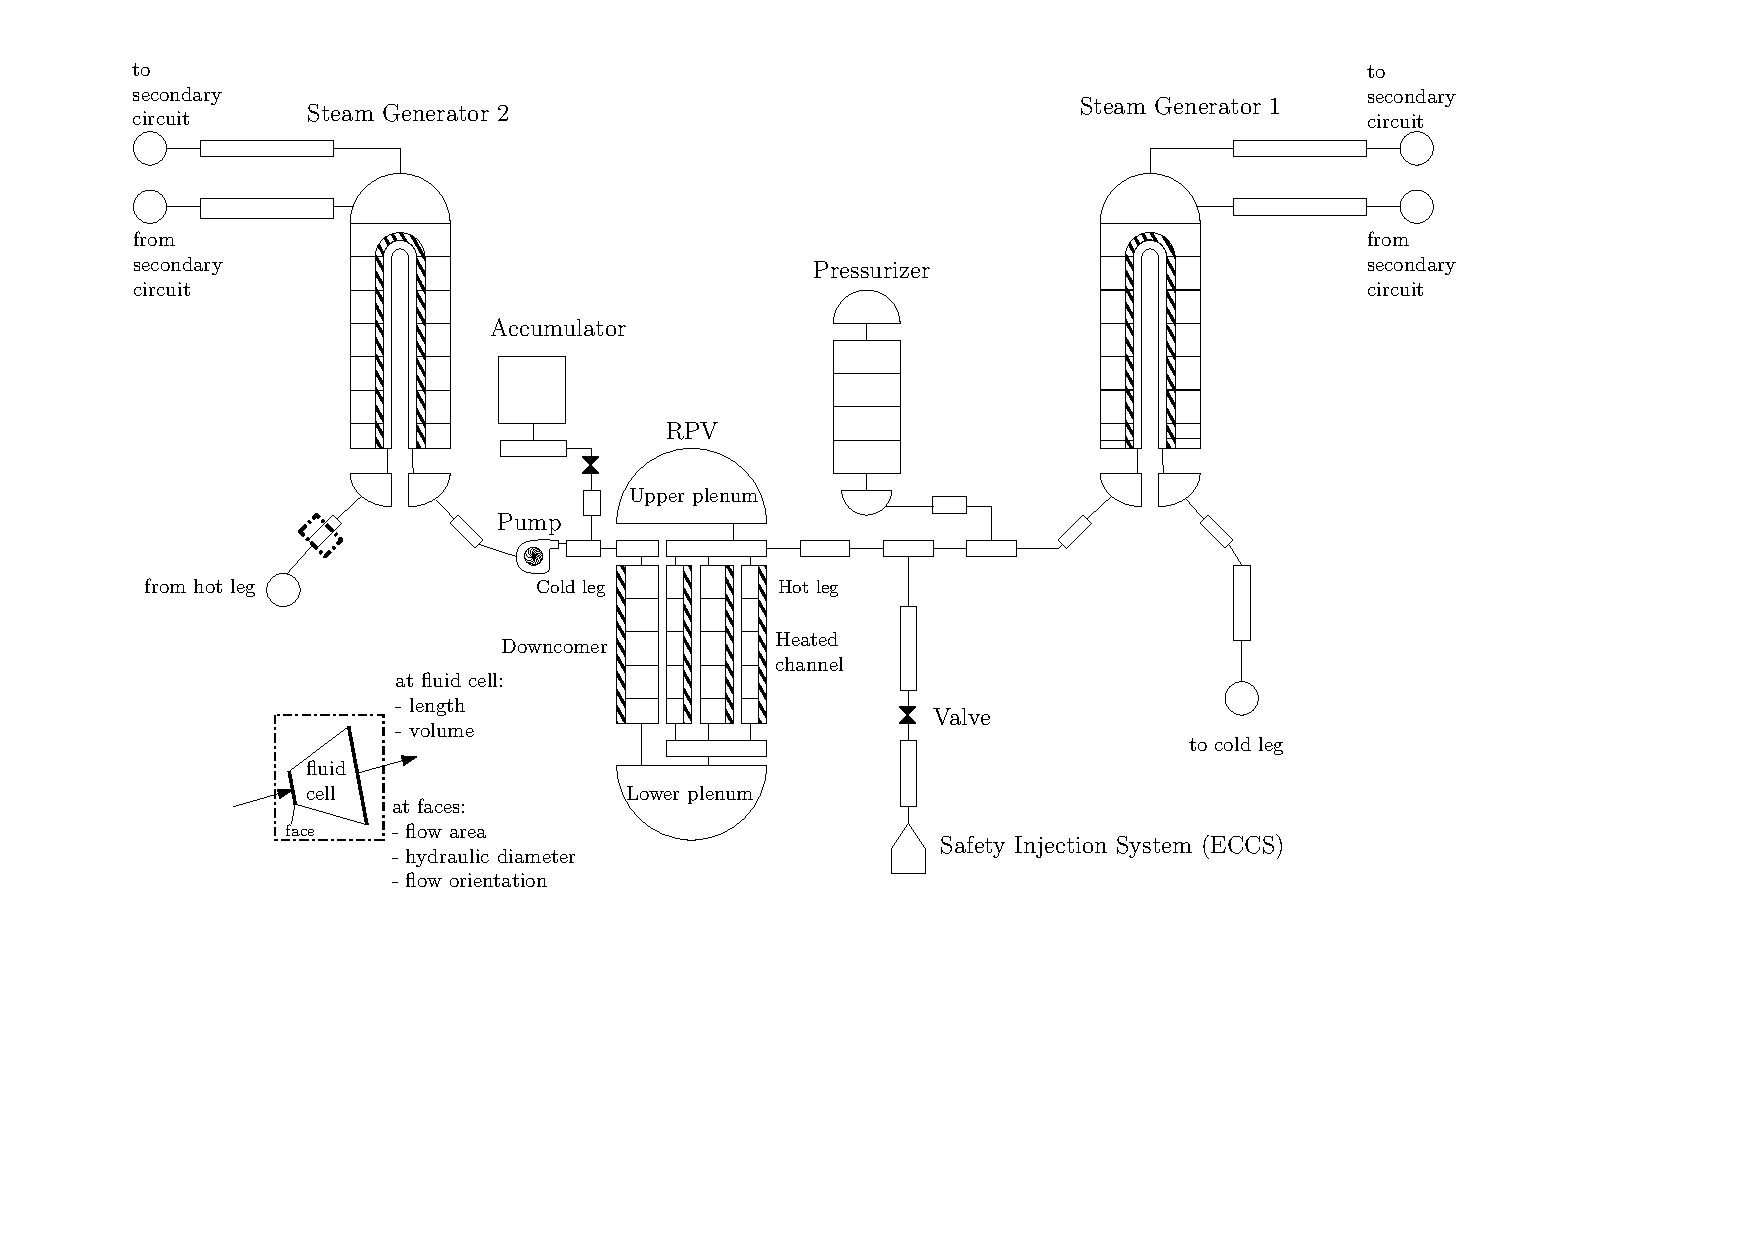
\includegraphics[width=\textwidth]{../figures/chapter1/figures/nodalization}
	\caption[Nodalization of a nuclear power plant (NPP) in a thermal-hydraulics (TH) system code]{Nodalization of an \gls[hyper=false]{npp} in a \glsfirst[hyper=false]{th} system code. Shaded elements are heated elements, where heat exchange occurs between the element and the fluid.}
	\label{fig:ch1_nodalization}
\end{figure}

% Structure of a system code
The typical structure of a system code is illustrated in Fig.~\ref{fig:ch1_th_system_code}.
As can be seen, system code constitutes of several building blocks that can be used to model and simulate wide ranges of systems and conditions.
\marginpar{Structure of thermal-hydraulics system codes}
It includes a set of conservation equations, closure laws, and equation of states.
System codes are complemented with models for special components that performs specific function (e.g., solid heated structure, pumps, and separators) or actions during transient (e.g., valves, instrumentation, and control systems);
and models for special processes and phenomena that are relevant to the conditions of \glspl[hyper=false]{lwr} but too complex to model implicitly in the (simplified) conservation equations (e.g., critical flow).
In fact, the inclusion of models for those components and processes relevant to the conditions of \glspl[hyper=false]{lwr} are the defining characteristics of \gls[hyper=false]{th} system code \cite{DAuria2012}.   
\begin{figure}[!bth]	
	\centering
	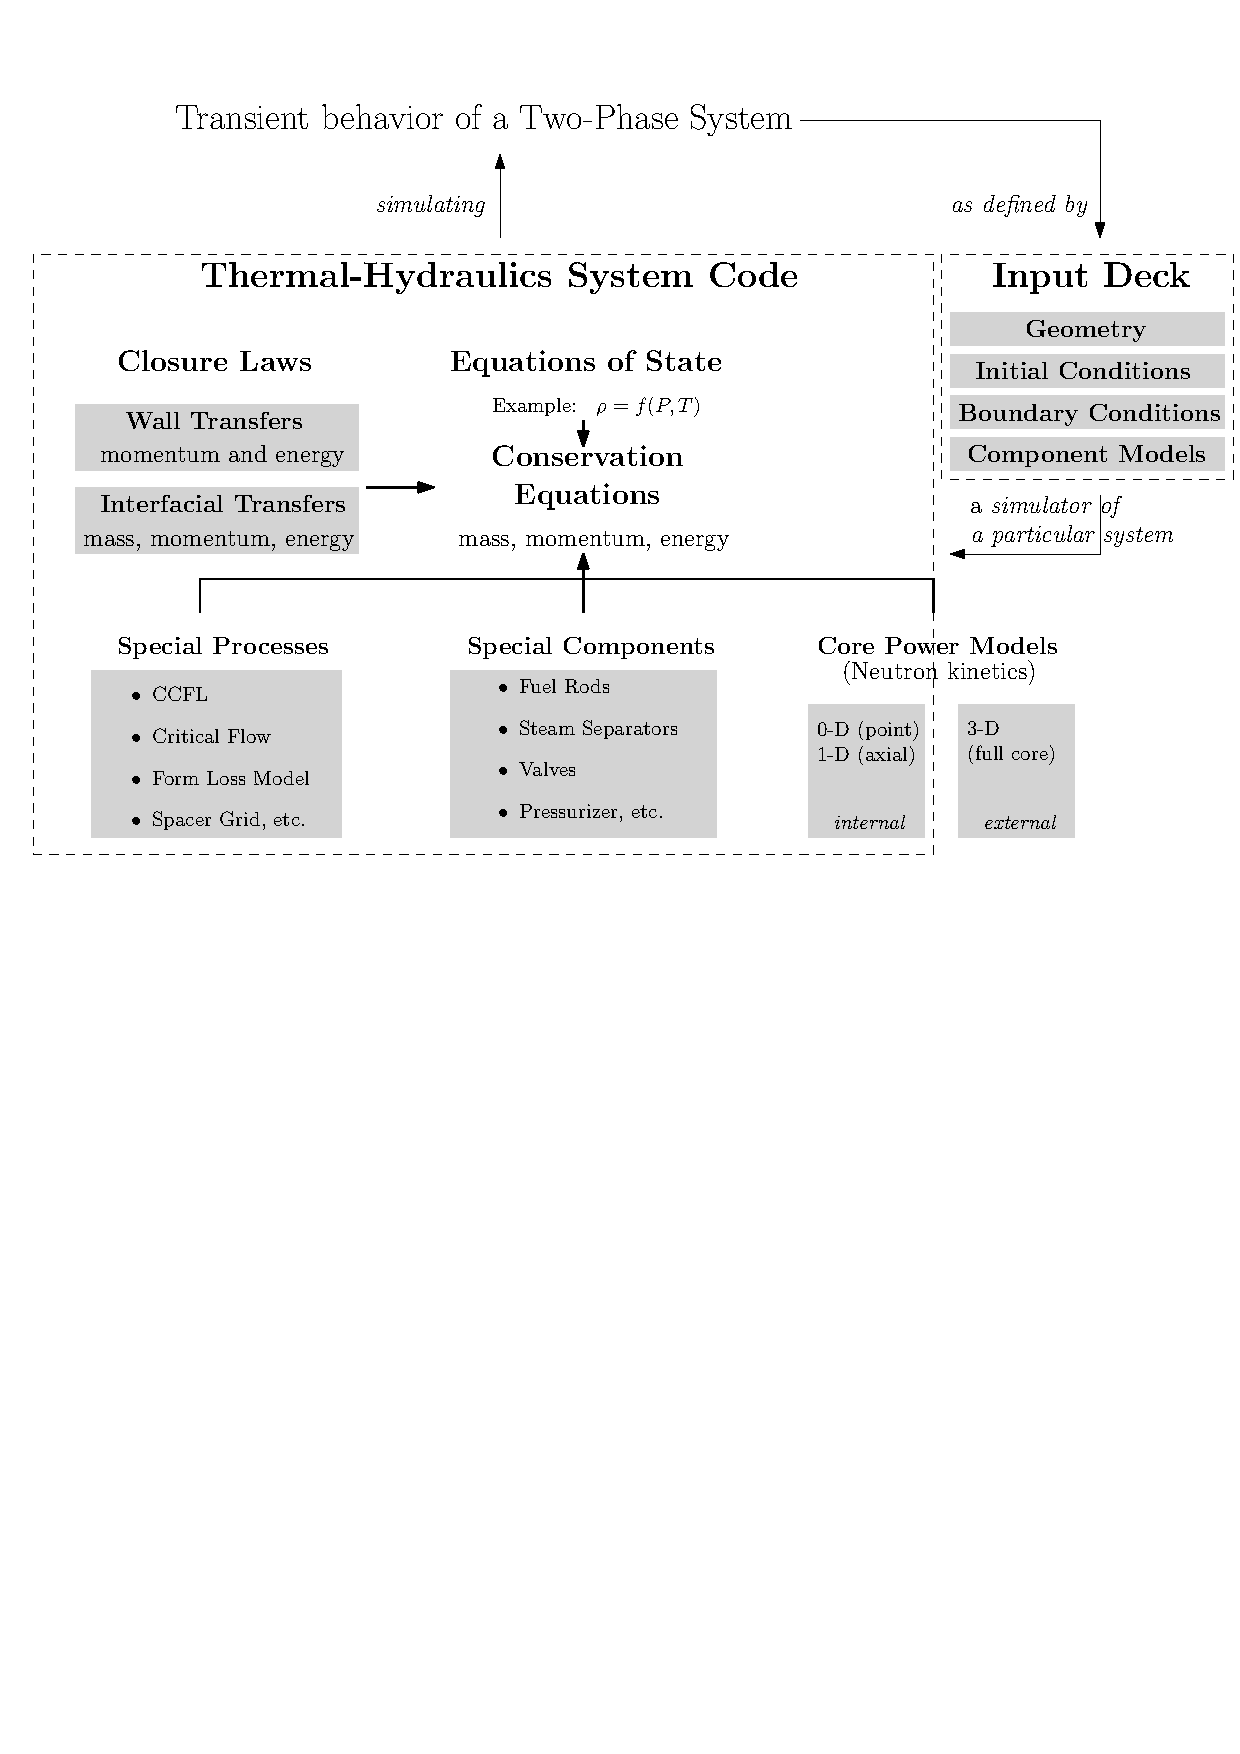
\includegraphics[width=\textwidth]{../figures/chapter1/figures/th_system_code}
	\caption[Generic structure of a thermal-hydraulics (TH) system code]{Generic structure of a \glsfirst[hyper=false]{th} system code. The code and a system specified by the input deck define a \emph{simulator} of that system.}
	\label{fig:ch1_th_system_code}
\end{figure}

% Constitutive Equations
The core element of a system code is a set of conservation equations describing the dynamics of the state variables of the fluid.
To close the system of equations (i.e., to have the same number of equations as the number of unknowns), it has to be complemented by two additional set of constitutive equations.
The first is the equation of state describing the thermodynamic relation between state variables of a given fluid.
The second is the closure relationships describing the interaction between phases and each phase to the boundary wall in terms of mass, momentum, and energy. 

% Two-fluid Model
The state-of-the-art model widely implemented in \gls[hyper=false]{th} system codes to describe the dynamics of fluid flow in \glspl[hyper=false]{npp} (specifically, \gls[hyper=false]{lwr}) is based on the \emph{two-fluid model}.
\marginpar{Two-fluid model}
This model separately treats the transport phenomena of the two-phases of fluid flow (gas and liquid) resulting in a set of six balance equations (mass, momentum, and energy for each of the two phases).
The model can capture phenomena where thermal and mechanical non-equilibrium conditions exist between the two phases, conditions which give more realistic pictures in a wide range of \gls[hyper=false]{npp} transients.

% Validity of Two-fluid Model
The validity of the two-fluid model widely implemented in thermal-hydraulics system codes relies on the proper modeling of the transfer terms between phases and between each phase and the boundary wall.
The transfer terms include interfacial drag, interfacial heat transfer, and wall heat transfer.
In principle, based on different two-phase flow patterns, different phase distributions and different interfacial structure can be observed.
As a result, each of these transfer terms takes different forms with different parameters depending on the pattern of the two-phase flow.
As the transfer terms represent different physical processes taking place for each flow pattern, they constitute the \emph{physical models} of a system code.

% Closure Laws, fully empirical
These physical models, or the so-called \emph{closure laws}, close the set of balance equations for mass, momentum, and energy of the two phases.
Based on their origins, closure laws can be classified into three categories: fully empirical, fully mechanistic, and semi-empirical \cite{Bestion2008}.
\marginpar{Closure laws origin}
Fully empirical are closure laws based only on the available representative experimental data by correlating transfer terms of interest with observed flow variables.
\marginpar{Fully empirical approach}
Given comprehensive experimental data, these models tend to be accurate within the range of experimental conditions (i.e., its validation domain).
On the other hand, an extrapolation outside of that range can give dubious results.

% fully mechanistic
Fully mechanistic (i.e., \emph{phenomenological}) approach for developing closure laws lies at the other end of the spectrum.
\marginpar{Fully mechanistic approach}
Using this approach, a physical mechanism that governs the phenomena of interest is postulated.
Experimental data plays a role only in validating such a postulated model.
If the model cannot be supported by the data then a complete revision might be required.
Mechanistic approach to closure laws modeling provides a scientific basis for prediction outside the validation data (i.e., extrapolation). 
However, its quality strongly depends on the adequacy of the postulated model and the associated assumptions in the first place.

% semi-empirical approach
Lastly, the semi-empirical approach combines both of the approach in the sense that a mechanistic model is initially developed based on a postulated governing mechanism.
\marginpar{Semi-empirical approach}
However, \emph{tuning} parameters are introduced that can be fitted to match the experimental data.
As such, these parameters become a measure of the inadequacy of the postulated model in explaining the data due to any missing physical processes, unaccounted for.

% Source of uncertainty
Any of these approaches proved to be a difficult effort \cite{Barre1990,Nelson1992,Wulff2007} due to various reasons ranging from lack of knowledge of the underlying physical process (with respect to the fully mechanistic modeling) to limitation in the amount of data as well as in measurement instruments (with respect to the fully empirical approach).
Simplifying assumptions and extrapolations are made because of these limitations.
In the end, closure laws in system codes are of mixed origins and they become a major source of uncertainty\footnote{defined in this thesis a state of limited knowledge, that is of \emph{epistemic} nature.} in the application of \gls[hyper=false]{th} system codes, especially when used outside their validation domains.
